\chapter{Results}
\label{ch:results}

The evaluation of the segmentation methodology that is proposed in this research was structured in a very progressive and the systemic manner which begins with the evaluation using synthetic phantom data and then extending into a very comprehensive analysis on real patient datasets. This layered evaluation approach allowed for a very detailed inspection of the model's behavior under controlled and also some clinically realistic conditions, which validates its robustness, generalization capability and the precision. The results were assessed using a number of statistical and validation techniques.

\section{Evaluation on Synthetic Phantom Data}
The first phase of the evaluation process involves the testing of the segmentation pipeline on simulated data, or so-called the phantoms, by introducing Poisson noise into the data using th x-cat phantom generator \cite{xcat}. Such a type of phantom is very widely regarded for the anatomical realism and is very frequently used in nuclear medicine as a gold standard baseline for the validation of the method. In this experiment varying levels of the Poisson noise were synthetically added to proper clean phantoms in order to simulate differing signal-to-noise ratio (SNR) conditions. The rationale behind the usage of Poisson noise is rooted in the fact that the nature of the SPECT imaging physics, where noise originates rom stochastic processes during the photon detection. This proves Poisson noise to be an appropriate and clinically relevant choice for the performance benchmarking of the models. The noise levels spanned a range from the severely degraded (low SNR) to relatively clean (high SNR), providing deep insights into the robustness of the algorithm against various levels of deteriorated image quality.

The quantitative analysis of the model on phantoms revealed that the proposed model maintains a performance above a random baseline across all the tested conditions but more importantly, it shows a notable increase in the segmentation accuracy, particularly after the 0 dB SNR as showed in \cref{Fig:noise}. While all the metrics showed an improvement with increasing SNR, one very significant result was the behavior of the precision of the model across the range. The precision showed 3x to 4x improvement compared to the other available metrics, showing that the model provides strong in selectivity in identifying relevant regions even in noisy volumes. This capability is very essential for clinical reliability, where the false positives could lead to unnecessary procedures.

\begin{figure}[htb!] % Changed from figure* to figure unless you specifically need double-column
\centering
% \begin{subfigure}[b]{1.5\textwidth} 
\centering
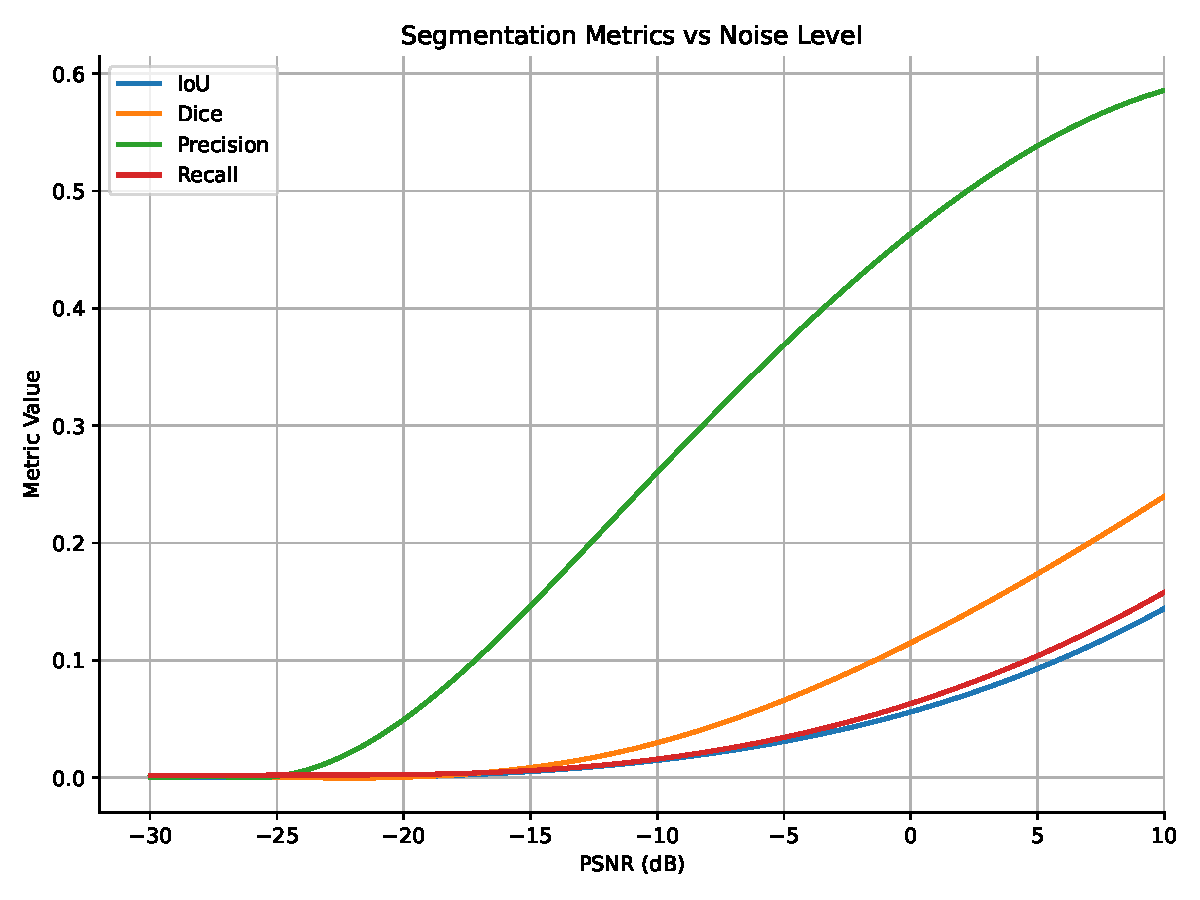
\includegraphics[width=1\textwidth]{images/metrics_vs_noise_cubic.pdf}
\caption{\centering Metric values against Noise in phantoms}
\label{Fig:noise}
\end{figure}

\section{Quantitative Comparison with Transformer Architectures}
In order to benchmark the proposed architecture against the state-of-the-art transformer based segmentation models we implemented two relevant and efficiently proved alternatives: nnFormer \cite{zhou2023nnformer} and Swin-UNETR \cite{10.1007/978-3-031-08999-2_22}. All of the models were trained under identical conditions using the same 60 patient training size and the 14 patient validation size in order to ensure a fair comparison between the models. The averaged quantitative results are summarized in Table \ref{tab:quantitative_comparison}. The proposed architecture consistently outperformed both the models for comparison across almost all the evaluation metrics. notably the precision, dice and the IoU score were higher which reflects an enhanced segmentation accuracy and spatial consistency. The one exception was the recall, where Swin-UNetR achieves a slightly higher values due to the consistent over-segmentation trend that is observed over several different samples. This suggests that while Swin-UNetR may be able to capture more positive instances, it does that at the cost of specificity which leads to a higher false positives rate. These results prove that the superior balance that needs to be achieved between the precision and the recall is done by the architecture proposed, which is an extremely important aspect of the clinical segmentation tasks in order to avoid both under and oversegmentation.

\begin{table}[h!t]
\begin{tabular}{ |p{2.3cm}|p{2.3cm}|p{2.3cm}|p{2.3cm}|p{2.3cm}|}
\hline
\multicolumn{5}{|c|}{Averaged performance metrics} \\
\hline
& Precision & Recall & IoU & Dice score \\
\hline
Our model & \textbf{0.714} & 0.7545 & \textbf{0.5706} & \textbf{0.7172} \\
\hline
nnFormer & 0.6819 & 0.6457 & 0.4715 & 0.6334 \\
\hline
SWIN-UNetR & 0.5329 & \textbf{0.9158} & 0.4949 & 0.6404 \\
\hline
\end{tabular}
\caption{Averaged segmentation results on the patient dataset. The proposed shape prior enhanced transformer is able to outperform the nnFormer \cite{zhou2023nnformer} and SWIN-transformer \cite{10.1007/978-3-031-08999-2_22} approaches in most metrics.}
\label{tab:quantitative_comparison}
\end{table}

\section{Effectiveness of Shape Priors on Anatomical Conformance}
More in-depth investigation into the role of SSP was conducted through a feature space analysis which is visualized in \cref{Fig:preds}. Contrary to the unbiased transformer models that rel completely on the features hierarchies that are learned, this method benefits from anatomical guidance which is embedded completely through the shape prior network. The visualizations confirm that the incorporation of prior-based optimization majorly improves the ability of the model to predict the boundaries of the LV. The optimization with this constraint which is introduced by the shape prior encourages better outcomes anatomically and also provides a better regularization for the learning process. These findings confirm the hypothesis that the use of SSP can guide the structural learning of the model resulting in better performance and easier interpretibility.

\begin{figure}[htbp]
\centering
\resizebox{0.7\textwidth}{!}{ % Control overall width here
\begin{tabular}{cccc} % 4 columns
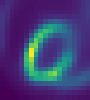
\includegraphics[width=0.22\textwidth]{images/segs/axial_input.png} &

\includegraphics[width=0.22\textwidth]{images/segs/axial_gt.png} &

\includegraphics[width=0.22\textwidth]{images/segs/axial_pred.png} &

\includegraphics[width=0.22\textwidth]{images/segs/axial_pred_SP.png} \\

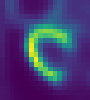
\includegraphics[width=0.22\textwidth]{images/segs/coronal_input.png} &

\includegraphics[width=0.22\textwidth]{images/segs/coronal_gt.png} &

\includegraphics[width=0.22\textwidth]{images/segs/coronal_pred.png} &

\includegraphics[width=0.22\textwidth]{images/segs/coronal_pred_SP.png} \\

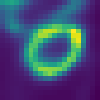
\includegraphics[width=0.22\textwidth]{images/segs/sagittal_input.png} &

\includegraphics[width=0.22\textwidth]{images/segs/sagittal_gt.png} &

\includegraphics[width=0.22\textwidth]{images/segs/sagittal_pred.png}&

\includegraphics[width=0.22\textwidth]{images/segs/sagittal_pred_SP.png} \\
\end{tabular}
}
\caption{Segmentation results, the first column depicts the source left ventricle volume, the second column is the ground truth labels. The third column shows the best performant competing model the nnFormer and the last is the proposed model's predicted left ventricle labels}
\label{Fig:preds}
\end{figure}

\section{Receiver Operating Characteristic (ROC) Analysis}
In order to assess the behavior of the segmentation model as a classifier-like model, a Receiver Operating Characteristic (ROC) curve was calculated on the test set of the patients, which is shown in \cref{Fig:roc}. ROC is a very well established method which helps to evaluate the discriminative power of a model. It works by plotting the true positive rate against the false positive rate across a number of thresholds. An interesting finding is the fact that the curve reveals a small fluctuation in the performance, which a one point dips below the threshold of the random classifier, which is 0.5, after the 0.75 mark. Upon very close examination of the model, this drop is found to be connected to the inconsistencies and the imperfections in the ground truth labels which were manually annotated and hence got subject to inter-observer variability.

\begin{equation}
\addcontentsline{equ}{equations}{\protect\numberline{\theequation}True Positive Rate}
\text{TPR} = \frac{TP}{TP + FN}
\end{equation}
\begin{equation}
\addcontentsline{equ}{equations}{\protect\numberline{\theequation}False Positive Rate}
\text{FPR} = \frac{FP}{FP + TN}
\end{equation}

This observation highlights the very essential role of the having the phase of quality control in the preparation of the dataset. Inconsistent labeling of the ground truths can lead to misleading evaluations, which strengthens the need for a standardized protocol of labeling or the usage ot multi-annotator consensus labels The ROC curve does not just evaluate the behavior of the model but also surfaced the underlying limitations that are present in the dataset, which adds value beyondd the traditional diagnostic use.

\begin{figure}[htb!] % Changed from figure* to figure unless you specifically need double-column
\centering
% \begin{subfigure}[b]{1.5\textwidth} 
\centering
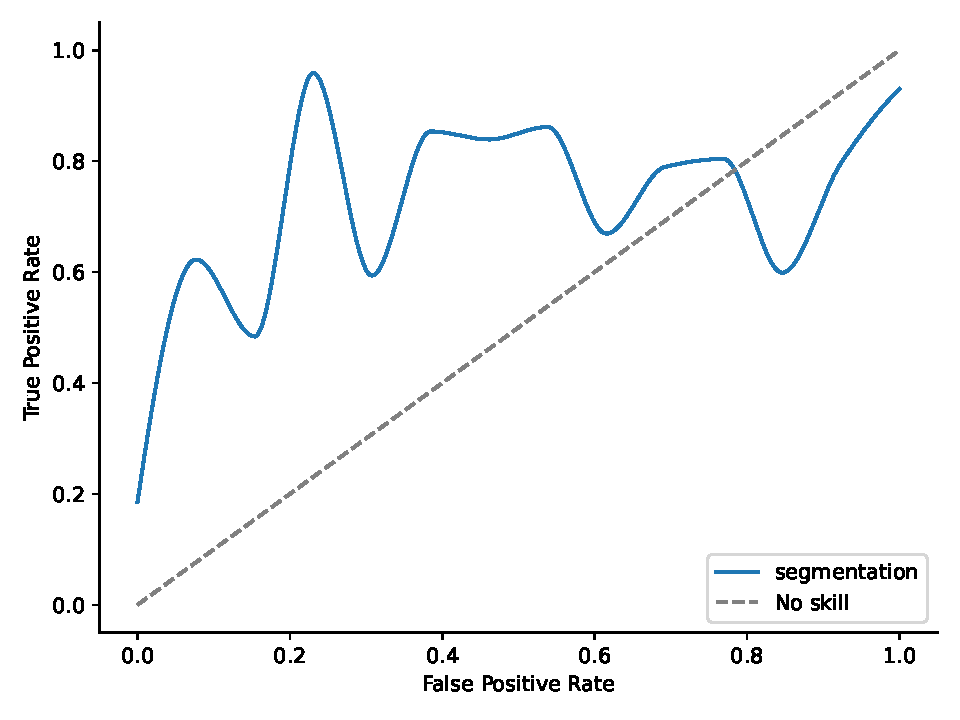
\includegraphics[width=1\textwidth]{images/ROC.pdf}
\caption{\centering ROC curve on test data}
\label{Fig:roc}
\end{figure}

\section{UMAP Embedding of Bottleneck Representations}
In order to gain further insights into the learned representations of the developed model, we performed a method of dimensionality reduction called the Uniform Manifold Approximation and Projection (UMAP) \cite{McInnes2018} on the bottleneck features that are extracted from the bottleneck as an output. We select five samples at random, each from the training and the test set and computed the UMAP projections using the configuration $(10, 0.1, \text{cosine}, 42)$, representing the number of neighbors, minimum distance, similarity measure, and random seed, respectively. As shown in \cref{Fig:umap train}, The embeddings from the training set show a high degree of coherence structurally, which indicates a well learned representation by the model internally. 

\begin{figure}[htb!] % Changed from figure* to figure unless you specifically need double-column
\centering
% \begin{subfigure}[b]{1.5\textwidth} 
\centering
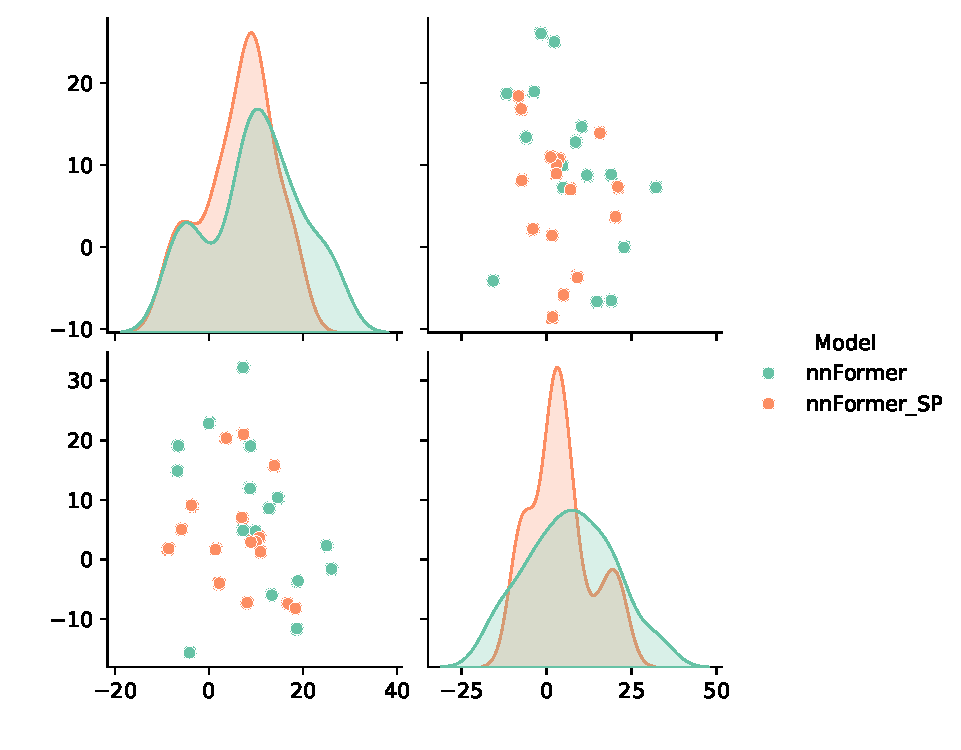
\includegraphics[width=1\textwidth]{images/Umap_train.pdf}
\caption{\centering UMAP bottleneck feature representation on training data}
\label{Fig:umap train}
\end{figure}

In contrast to this the embeddings on the test set which are visualized in \cref{Fig:umap test} were more dispersed from the nnFormer baseline model but were a lot more compact and structured for the proposed model. This difference show that the inclusion of the SSP contribute to having a lot more stable and generalizable latent representation even on data that is previously unseen. The ability of the model to perform discriminatively and have consistent latent space representation is a major indicator of the strength of generalization in the performance of the model. These results further prove that the qualitative and the also the quantitative improvements that are gained through the anatomical regularization is very beneficial.

\begin{figure}[htb!] % Changed from figure* to figure unless you specifically need double-column
\centering
% \begin{subfigure}[b]{1.5\textwidth} 
\centering
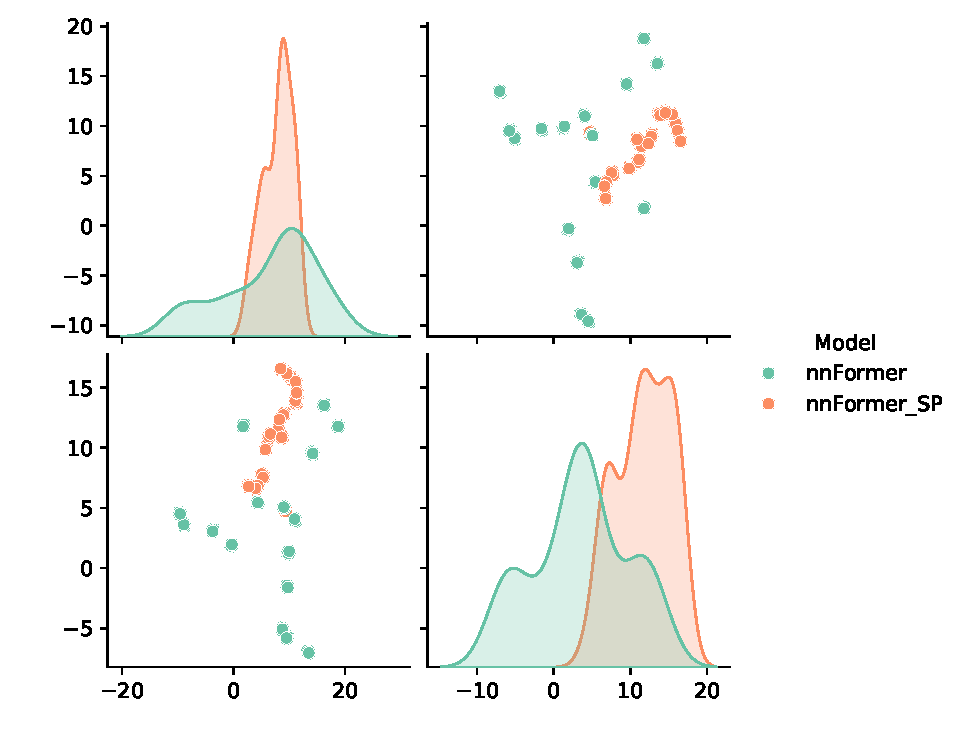
\includegraphics[width=1\textwidth]{images/Umap_test.pdf}
\caption{\centering UMAP bottleneck feature representation on testing data}
\label{Fig:umap test}
\end{figure}

\section{Training with Varying Dataset Sizes}
To evaluate the efficiency of the learning of the model even further, and also to understand the data requirements of the proposed architecture an additional series of experiments was conducted in which both the baseline nnFormer model and the nnFormer model improved with the SSP were trained progressively on increasing subsets of the training data. The sizes of the subsets included 10, 20, 30, 40, 50, and 60 patients. Each of the subsets was constructed randomly by taking a random sample from the full training dataset while ensuring consistent data preprocessing. For each of these subsets, the models were trained from scratch using the same hyperparameters, optimizer settings, and the augmentations which are described in the methodology chapter in detail. The goal of the experiments was to measure the performance gains as a functions of the dataset size and to asses how effectively the models could generalize rom the limited amount of training data. The performance of the models was measured on the full test set using four different key metrics: Dice coefficient, Recall, Precision and the IoU score. These results are summarized into a set of bar charts for each of the metrics, illustrated in \cref{Fig:datasets}. These plots provide a very detailed view of the relationship between the size of the training set ans the performance of the model. As expected both the models show improvements in all the metrics as the size of the training set increases. However, the nnFormerSP consistently outperforms the baseline nnFormer at every stage of the training size. In the smaller subset size, the performance of the models are very inconsistent and random, the nnFormer baseline achieved a higher precision but the nnFormerSP achieves a higher score for each of the other 3 metrics, with having a huge difference in the values this alone proves the strength of incorporating shape priors in the training of the models and that it effectively compensates for the limited amount of training data. As the dataset size approaches patients,the performance of both the models are more consistent and stable and converge closer together but the nnFormerSP still retains a clear edge over the baseline in having better consistency and segmentation ability. These results further prove the advantage of using SSP in not only low-data settings but also in boosting the overall performance of the model across varying training conditions. This experiment highlights the value of the shape-based regularization in DL pipelines, specifically in medical imaging especially when the availability of large amount of annotated data is difficult.

\begin{figure}[htb!] % Changed from figure* to figure unless you specifically need double-column
\centering
% \begin{subfigure}[b]{1.5\textwidth} 
\centering
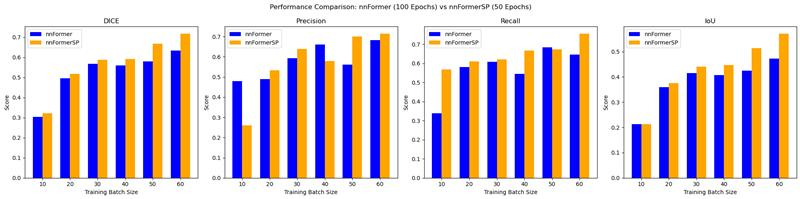
\includegraphics[width=1\textwidth]{images/datasets.jpeg}
\caption{\centering Evaluation metric variation based on dataset size}
\label{Fig:datasets}
\end{figure}

\section{Conclusion of Results}
The rsults of all the performed experiments demonstrate a very clear and a constant advantage of the proposed methodology over the baseline and other comparative approaches. From the synthetic noise resilience to the clinical accuracy on the real life patient data, the model proposed in the research not only delivers a higher performance in segmentation tasks but also introduces a reliability anatomically and strength of generalizablity through the use of statistical shape priors. These attributes of a model are essential for the practical deployment of the segmentation tools in any real-world clinical settings.
